\documentclass[12pt,a4paper]{report}

% --- Packages ----------------------------------------------------------------
\usepackage[utf8]{inputenc}
\usepackage[T1]{fontenc}
\usepackage[italian]{babel}
\usepackage{geometry}
\usepackage{graphicx}
\usepackage{amsmath}
\usepackage{hyperref}
\usepackage{booktabs}
\usepackage{longtable}
\usepackage{array}
\usepackage{xcolor}
\usepackage{listings}
\usepackage{fancyhdr}
\usepackage{titlesec}
\usepackage{tcolorbox}
\usepackage{enumitem}
\usepackage{float}
\usepackage{caption}
\usepackage{microtype}
\usepackage{parskip}
\usepackage{palatino}
\usepackage{tabularx}
\usepackage{tikz}
\usetikzlibrary{shapes.geometric, arrows.meta, positioning}

\geometry{
  top=2.5cm, bottom=2.5cm,
  left=3cm,  right=3cm
}

% --- Liste compatte ----------------------------------------------------------
\setlist[itemize]{itemsep=3pt, parsep=2pt, topsep=4pt}
\setlist[enumerate]{itemsep=3pt, parsep=2pt, topsep=4pt}

% --- Colors ------------------------------------------------------------------
\definecolor{agentblue}{RGB}{30,80,160}
\definecolor{agentdark}{RGB}{18,50,100}
\definecolor{lightgray}{RGB}{245,245,245}
\definecolor{darkgray}{RGB}{80,80,80}
\definecolor{codebg}{RGB}{248,248,248}
\definecolor{bordercolor}{RGB}{200,200,200}
\definecolor{boxheader}{RGB}{50,50,50}
\definecolor{chaptercolor}{RGB}{25,65,140}
\definecolor{rulecolor}{RGB}{180,200,230}
\definecolor{tableheader}{RGB}{235,242,252}
\definecolor{colorhigh}{RGB}{200,40,40}
\definecolor{colormedium}{RGB}{200,130,20}
\definecolor{colorok}{RGB}{30,130,60}

% --- Hyperref ----------------------------------------------------------------
\hypersetup{
  colorlinks=true,
  linkcolor=agentblue,
  urlcolor=agentblue,
  citecolor=agentblue,
  pdftitle={Agent 2 - Casi di Test},
  pdfauthor={Intelligent Domain Architect Team}
}

% --- tcolorbox styles --------------------------------------------------------
\tcbuselibrary{skins,breakable}

\newtcolorbox{technicalbox}[1]{
  enhanced,
  title={#1},
  colback=lightgray,
  colframe=agentblue!70!black,
  colbacktitle=agentblue,
  coltitle=white,
  fonttitle=\small\bfseries\sffamily,
  breakable,
  boxrule=0.6pt,
  arc=3pt,
  left=8pt, right=8pt, top=6pt, bottom=6pt,
  shadow={1pt}{-1pt}{0pt}{black!15}
}

\newtcolorbox{issuebox}[2]{
  enhanced,
  title={#1},
  colback=lightgray,
  colframe=#2,
  colbacktitle=#2,
  coltitle=white,
  fonttitle=\small\bfseries\sffamily,
  breakable,
  boxrule=0.6pt,
  arc=3pt,
  left=8pt, right=8pt, top=6pt, bottom=6pt
}

\newtcolorbox{outputbox}[1]{
  enhanced,
  title={#1},
  colback=codebg,
  colframe=darkgray!60,
  colbacktitle=darkgray,
  coltitle=white,
  fonttitle=\small\bfseries\sffamily,
  breakable,
  boxrule=0.6pt,
  arc=3pt,
  left=8pt, right=8pt, top=6pt, bottom=6pt
}

% --- Listings ----------------------------------------------------------------
\lstset{
  basicstyle=\ttfamily\footnotesize,
  backgroundcolor=\color{codebg},
  frame=single,
  framesep=6pt,
  xleftmargin=8pt,
  xrightmargin=8pt,
  rulecolor=\color{agentblue!30},
  breaklines=true,
  breakatwhitespace=true,
  showstringspaces=false,
  tabsize=2,
  captionpos=b,
  numbers=none
}

% --- Captions ----------------------------------------------------------------
\captionsetup{
  font=small,
  labelfont={bf,color=agentblue},
  textfont={it},
  skip=8pt
}

% --- Headers/Footers ---------------------------------------------------------
\pagestyle{fancy}
\setlength{\headheight}{16pt}
\fancyhf{}
\fancyhead[L]{\small\textcolor{agentblue}{\textit{Agent 2 -- Consistency \& Conflict Analyzer}}}
\fancyhead[R]{\small\textcolor{darkgray}{\textit{Casi di Test}}}
\fancyfoot[C]{\textcolor{darkgray}{\thepage}}
\renewcommand{\headrulewidth}{0.4pt}
\renewcommand{\headrule}{\hbox to\headwidth{\color{rulecolor}\leaders\hrule height \headrulewidth\hfill}}

% --- Chapter/Section titles --------------------------------------------------
\titleformat{\chapter}[display]
  {\normalfont\huge\bfseries\color{chaptercolor}}
  {\tikz[remember picture,overlay]\node[fill=agentblue,text=white,
    minimum width=2.5cm,minimum height=2.5cm,font=\fontsize{50}{60}\selectfont\bfseries,
    inner sep=0pt] at ([xshift=1.25cm,yshift=-1.25cm]current page.north west|-0,0)
    {\thechapter}; \hspace{2.8cm}\textcolor{darkgray}{\Large\MakeUppercase{\chaptertitlename}}}
  {10pt}{\Huge}
  [\vspace{-5pt}{\color{rulecolor}\titlerule[2pt]}]

\titleformat{\section}
  {\normalfont\Large\bfseries\color{agentblue}}{\thesection}{1em}{}
  [\vspace{-5pt}{\color{rulecolor}\titlerule[0.6pt]}]

\titleformat{\subsection}
  {\normalfont\large\bfseries\color{agentdark}}{\thesubsection}{1em}{}

% -----------------------------------------------------------------------------
\raggedbottom

\begin{document}

% --- Title Page --------------------------------------------------------------
\begin{titlepage}
  \begin{tikzpicture}[remember picture,overlay]
    \fill[agentblue] (current page.north west) rectangle
      ([xshift=1.2cm]current page.south west);
    \fill[agentblue!80] ([yshift=-3cm]current page.north west) rectangle
      ([yshift=-3.08cm]current page.north east);
    \fill[agentblue!80] ([yshift=3cm]current page.south west) rectangle
      ([yshift=3.08cm]current page.south east);
  \end{tikzpicture}

  \centering
  \vspace*{0.8cm}
  {\large\textbf{\textcolor{agentblue}{Università Campus Bio-Medico di Roma}}\\[4pt]}
  {\normalsize Facoltà di Ingegneria\\[2pt]}
  {\normalsize Corso di Laurea in Ingegneria dei Sistemi Intelligenti\\}
  \vspace{3cm}
  {\color{rulecolor}\rule{0.6\textwidth}{1.5pt}}\\[0.8cm]
  {\Huge\textbf{\textcolor{agentblue}{Agent 2}}}\\[0.5cm]
  {\LARGE\textbf{\textcolor{agentdark}{Consistency \& Conflict Analyzer}}}\\[0.5cm]
  {\color{rulecolor}\rule{0.6\textwidth}{1.5pt}}\\[1cm]
  {\large Casi di Test:\\[0.3cm]
  \textit{Scenari di validazione, problemi attesi e output del sistema}}

  \vfill

  \begin{minipage}[t]{0.45\textwidth}
    {\small\textcolor{darkgray}{\textit{Studenti:}}}\\[4pt]
    Claudio \textbf{Dragotta}\\
    Matteo \textbf{Grande}
  \end{minipage}
  \hfill
  \begin{minipage}[t]{0.45\textwidth}
    \raggedleft
    {\small\textcolor{darkgray}{\textit{Docenti:}}}\\[4pt]
    Ing.\ Floriano Caprio \\
    Dott.\ Ing. Ermanno Cordelli
  \end{minipage}

  \vspace{1.5cm}
  {\color{rulecolor}\rule{0.4\textwidth}{0.8pt}}\\[6pt]
  {\normalsize Anno Accademico 2025/2026}
\end{titlepage}

% --- ToC ---------------------------------------------------------------------
\tableofcontents
\clearpage

% =============================================================================
\chapter{Panoramica dei Casi di Test}
% =============================================================================

\section{Introduzione}

L'\textbf{Agent 2 -- Consistency \& Conflict Analyzer} è il secondo nodo della pipeline
\textit{Intelligent Domain Architect}. Il suo compito è analizzare un \textit{domain model}
in formato JSON (prodotto dall'Agent~1) e rilevare automaticamente le incoerenze
semantiche, i conflitti tra requisiti e le violazioni delle regole Domain-Driven Design (DDD).

I casi di test qui documentati sono stati progettati per:
\begin{itemize}
  \item verificare la correttezza del motore di analisi su scenari noti;
  \item coprire tutti e \textbf{7 tipi di problema} rilevabili dall'agente;
  \item testare domini applicativi distinti (e-commerce, sanità, finanza);
  \item garantire l'assenza di falsi positivi su un modello DDD corretto.
\end{itemize}
\clearpage
\section{Tipologie di Problemi Rilevati}

L'agente rileva sette categorie di incoerenza, classificate per severità:

\begin{table}[H]
\centering
\renewcommand{\arraystretch}{1.4}
\begin{tabularx}{\textwidth}{l l X}
\toprule
\textbf{Tipo} & \textbf{Severità} & \textbf{Descrizione} \\
\midrule
\texttt{ENTITY\_OVERLAP} & \textcolor{colorhigh}{HIGH} &
  La stessa entità è definita in più Bounded Context senza un proprietario chiaro \\
\texttt{REQUIREMENT\_CONFLICT} & \textcolor{colorhigh}{HIGH} &
  Due requisiti funzionali si contraddicono logicamente \\
\texttt{DUPLICATE\_EVENT} & \textcolor{colorhigh}{HIGH} &
  Lo stesso evento di dominio è emesso da più servizi distinti \\
\texttt{INCOMPATIBLE\_PATTERN} & \textcolor{colorhigh}{HIGH} &
  Un pattern di comunicazione è incompatibile con i requisiti di consistenza \\
\texttt{SEMANTIC\_AMBIGUITY} & \textcolor{colormedium}{MEDIUM} &
  Un termine è usato con significati diversi in contesti diversi \\
\texttt{NAMING\_VIOLATION} & \textcolor{colormedium}{MEDIUM} &
  Un evento non rispetta la convezione \texttt{<Aggregato><VerboPastato>} \\
\texttt{MISCLASSIFIED\_DOMAIN} & \textcolor{colormedium}{MEDIUM} &
  Un dominio è classificato erroneamente (es.\ Generic classificato come Core) \\
\bottomrule
\end{tabularx}
\caption{Tipologie di problema rilevabili da Agent~2}
\label{tab:issue-types}
\end{table}

\section{Riepilogo dei Casi di Test}

\begin{table}[H]
\centering
\renewcommand{\arraystretch}{1.4}
\begin{tabularx}{\textwidth}{l l X c c}
\toprule
\textbf{\#} & \textbf{File} & \textbf{Scenario} & \textbf{Problemi} & \textbf{Scopo} \\
\midrule
1 & \texttt{example\_good.json}    & E-Commerce (corretto) & 0  & Baseline \\
2 & \texttt{example\_demo.json}    & E-Commerce (demo)     & 3  & Demo rapida \\
3 & \texttt{example\_bad.json}     & E-Commerce (stress)   & 13 & Stress test \\
4 & \texttt{case\_healthcare.json} & Gestione Ospedaliera  & 4  & Dominio sanità \\
5 & \texttt{case\_banking.json}    & Digital Banking       & 4  & Dominio finanza \\
\bottomrule
\end{tabularx}
\caption{Riepilogo dei cinque casi di test}
\label{tab:test-summary}
\end{table}

\clearpage

% =============================================================================
\chapter{Caso 1 --- \texttt{example\_good.json}}
% =============================================================================

\section{Descrizione del Scenario}

\begin{technicalbox}{Scenario: E-Commerce Platform --- Modello Corretto}
Modello DDD completo di una piattaforma e-commerce progettata secondo le best practice.
Utilizzato come \textbf{baseline di riferimento} per verificare l'assenza di falsi positivi.
\end{technicalbox}

\section{Struttura del Dominio}

\begin{table}[H]
\centering
\renewcommand{\arraystretch}{1.3}
\begin{tabularx}{\textwidth}{l l X}
\toprule
\textbf{Tipo} & \textbf{Nome} & \textbf{Responsabilità} \\
\midrule
Core       & Order Management      & Gestione del ciclo di vita degli ordini \\
Core       & Product Catalog       & Catalogo prodotti e prezzi \\
Supporting & Payment Processing    & Elaborazione pagamenti \\
Supporting & Shipping              & Spedizione e tracking \\
Supporting & Customer Management   & Profilo cliente e indirizzi \\
Supporting & Inventory             & Gestione scorte e riserve \\
Generic    & Notification Service  & Invio notifiche (email, SMS) \\
Generic    & Authentication \& Auth & Autenticazione e autorizzazione \\
\bottomrule
\end{tabularx}
\caption{Domini del caso \texttt{example\_good.json}}
\label{tab:good-domains}
\end{table}

\begin{technicalbox}{Caratteristiche del Modello Corretto}
\begin{itemize}
  \item Ogni entità appartiene a \textbf{un solo} Bounded Context
  \item Tutti gli eventi sono nominati al passato (\texttt{OrderCreated}, \texttt{PaymentAuthorized}, \texttt{ShipmentDispatched})
  \item Ogni evento ha \textbf{un unico emittente}
  \item I requisiti di consistenza sono compatibili tra loro
  \item Le integrazioni tra contesti usano pattern documentati (\textit{event-driven}, \textit{open-host-service})
  \item Authentication è correttamente classificato come dominio \textit{Generic}
  \item Il Shared Kernel contiene solo Value Objects condivisi (\texttt{Money}, \texttt{Address})
\end{itemize}
\end{technicalbox}

\section{Scopo del Test}

Verificare che l'agente \textbf{non produca falsi positivi} su un modello correttamente progettato.
La pipeline deve terminare con stato \texttt{VALID} senza generare domande di chiarimento.

\section{Output Atteso}

\begin{outputbox}{Risposta dell'agente}
\begin{lstlisting}
{
  "status": "VALID",
  "summary": {
    "total_issues": 0
  },
  "follow_up_questions": []
}
\end{lstlisting}
\end{outputbox}

\clearpage

% =============================================================================
\chapter{Caso 2 --- \texttt{example\_demo.json}}
% =============================================================================

\section{Descrizione del Scenario}

\begin{technicalbox}{Scenario: E-Commerce Platform --- Demo Interattiva}
Modello e-commerce con \textbf{3 problemi intenzionali} scelti per rappresentare le categorie
principali di incoerenza. Questo caso è stato utilizzato nella demo interattiva con n8n
presentata al professore.
\end{technicalbox}

\section{Struttura del Dominio}

Tre domini Core: \textbf{Order Management}, \textbf{Product Catalog}, \textbf{Inventory}.

\section{Problemi Intenzionali}

\subsection{Problema 1 --- ENTITY\_OVERLAP}

\begin{issuebox}{ENTITY\_OVERLAP --- Severità: HIGH}{colorhigh}
\begin{description}[leftmargin=3cm, labelwidth=2.8cm]
  \item[Entità]    \texttt{Product}
  \item[Contesti]  \texttt{OrderContext} e \texttt{CatalogContext}
  \item[Problema]  L'entità \texttt{Product} è definita in entrambi i contesti.
                   Non è chiaro quale dei due sia il proprietario.
  \item[Regola DDD] In DDD ogni entità deve appartenere a un solo Bounded Context;
                   gli altri vi accedono tramite riferimento (\texttt{ProductId}).
\end{description}
\end{issuebox}

\subsection{Problema 2 --- REQUIREMENT\_CONFLICT}

\begin{issuebox}{REQUIREMENT\_CONFLICT --- Severità: HIGH}{colorhigh}
\begin{description}[leftmargin=3cm, labelwidth=2.8cm]
  \item[Requisiti] \textbf{FR-ORD-001} vs \textbf{FR-ORD-002}
  \item[FR-ORD-001] \textit{``Un ordine è immutabile dopo la conferma''}
  \item[FR-ORD-002] \textit{``Un ordine può essere modificato entro 24 ore''}
  \item[Conflitto]  I due requisiti si contraddicono logicamente: l'ordine non
                   può essere contemporaneamente immutabile e modificabile.
\end{description}
\end{issuebox}

\subsection{Problema 3 --- DUPLICATE\_EVENT}

\begin{issuebox}{DUPLICATE\_EVENT --- Severità: HIGH}{colorhigh}
\begin{description}[leftmargin=3cm, labelwidth=2.8cm]
  \item[Evento]    \texttt{OrderCreated}
  \item[Emittenti] \texttt{order-management} e \texttt{product-catalog}
  \item[Problema]  Lo stesso evento viene emesso da due servizi distinti.
                   Questo crea ambiguità sui consumatori e può causare
                   elaborazioni duplicate nei sistemi downstream.
\end{description}
\end{issuebox}

\section{Scopo del Test}

Mostrare il comportamento dell'agente in una sessione interattiva con un numero
limitato di problemi facilmente spiegabili. Il loop domanda-risposta deve convergere
in 1--2 iterazioni.

\section{Output Atteso}

\begin{outputbox}{Risposta dell'agente}
\begin{lstlisting}
{
  "status": "ISSUES_FOUND",
  "summary": {
    "total_issues": 3,
    "entity_overlaps": 1,
    "requirement_conflicts": 1,
    "duplicate_events": 1
  },
  "follow_up_questions": [3 domande di chiarimento],
  "suggested_max_iterations": 2
}
\end{lstlisting}
\end{outputbox}

\clearpage

% =============================================================================
\chapter{Caso 3 --- \texttt{example\_bad.json}}
% =============================================================================

\section{Descrizione del Scenario}

\begin{technicalbox}{Scenario: E-Commerce Platform --- Stress Test}
Modello e-commerce con \textbf{13 problemi intenzionali} che coprono tutti e 7 i tipi
di errore rilevabili. Usato come stress test del motore di analisi per verificarne
la completezza e la robustezza.
\end{technicalbox}

\section{Struttura del Dominio}

\begin{table}[H]
\centering
\renewcommand{\arraystretch}{1.3}
\begin{tabularx}{\textwidth}{l.5 l.5 X}
\toprule
\textbf{Tipo} & \textbf{Nome} & \textbf{Nota} \\
\midrule
Core       & Order Management  & \\
Core       & Product Catalog   & \\
Core       & Authentication    & \textcolor{colorhigh}{Classificazione errata (dovrebbe essere Generic)} \\
Supporting & Payment Processing & \\
Supporting & Shipping           & \\
Supporting & Customer Management & \\
Supporting & Inventory          & \\
\bottomrule
\end{tabularx}

\caption{Domini del caso \texttt{example\_bad.json}}
\label{tab:bad-domains}
\end{table}
\clearpage
\section{Problemi Intenzionali}

\subsection{ENTITY\_OVERLAP (2 istanze)}

\begin{issuebox}{ENTITY\_OVERLAP \#1 --- Severità: HIGH}{colorhigh}
\textbf{Entità:} \texttt{Product} \\
\textbf{Contesti:} Order Management + Product Catalog \\
Definita in entrambi i contesti senza un owner dichiarato.
\end{issuebox}

\vspace{0.5em}

\begin{issuebox}{ENTITY\_OVERLAP \#2 --- Severità: HIGH}{colorhigh}
\textbf{Entità:} \texttt{Customer} \\
\textbf{Contesti:} Order Management + Customer Management \\
Definita in entrambi i contesti senza un owner dichiarato.
\end{issuebox}

\subsection{REQUIREMENT\_CONFLICT (3 istanze)}

\begin{table}[H]
\centering
\renewcommand{\arraystretch}{1.4}
\begin{tabularx}{\textwidth}{l X}
\toprule
\textbf{Requisiti in Conflitto} & \textbf{Descrizione del Conflitto} \\
\midrule
FR-ORD-002 vs FR-ORD-003 & Prezzo immutabile dopo conferma vs applicazione retroattiva di coupon \\
FR-ORD-002 vs FR-CAT-002 & Prezzo immutabile nell'ordine vs aggiornamenti di prezzo nel catalogo \\
FR-ORD-004 vs architettura & Strong consistency richiesta vs architettura solo event-driven (eventual consistency) \\
\bottomrule
\end{tabularx}
\caption{Conflitti tra requisiti in \texttt{example\_bad.json}}
\label{tab:req-conflicts}
\end{table}
\subsection{Semantic Ambiguity (due istanze)}

\begin{table}[H]
\centering
\renewcommand{\arraystretch}{1.3}
\begin{tabularx}{\textwidth}{l X X}
\toprule
\textbf{Termine} & \textbf{Contesti} & \textbf{Ambiguità} \\
\midrule
\texttt{Transaction} &
Order Management, Payment Processing &
Indica un movimento contabile in un contesto e un'operazione di pagamento nell'altro. \\

\texttt{Item} &
Order, Catalog, Shipping, Inventory (4 contesti) &
Usato con significati distinti nei diversi contesti applicativi. \\
\bottomrule
\end{tabularx}
\caption{Ambiguità semantiche identificate in \texttt{example\_bad.json}}
\label{tab:semantic_ambiguity}
\end{table}

\subsection{DUPLICATE\_EVENT (1 istanza)}

\begin{issuebox}{DUPLICATE\_EVENT --- Severità: HIGH}{colorhigh}
\textbf{Evento:} \texttt{OrderCreated} \\
\textbf{Emittenti:} \texttt{order-management} e \texttt{product-catalog}
\end{issuebox}

\subsection{NAMING\_VIOLATION (3 istanze)}

\begin{table}[H]
\centering
\renewcommand{\arraystretch}{1.4}
\begin{tabularx}{\textwidth}{l X l}
\toprule
\textbf{Evento Attuale} & \textbf{Problema} & \textbf{Nome Corretto} \\
\midrule
\texttt{ProcessPayment} & Verbo all'infinito, non al passato & \texttt{PaymentProcessed} \\
\texttt{ShipOrder}      & Verbo all'infinito, non al passato & \texttt{OrderShipped} \\
\texttt{Update}         & Troppo generico                    & \texttt{StockUpdated} \\
\bottomrule
\end{tabularx}
\caption{Violazioni di naming in \texttt{example\_bad.json}}
\label{tab:naming}
\end{table}

\subsection{INCOMPATIBLE\_PATTERN (1 istanza)}

\begin{issuebox}{INCOMPATIBLE\_PATTERN --- Severità: HIGH}{colorhigh}
\textbf{Requisito:} FR-PAY-002 richiede verifica \textit{real-time sincrona} dei pagamenti \\
\textbf{Pattern definito:} Solo \texttt{pub/sub} asincrono \\
\textbf{Problema:} Un requisito sincrono non può essere soddisfatto con sola comunicazione asincrona.
\end{issuebox}

\subsection{MISCLASSIFIED\_DOMAIN (1 istanza)}

\begin{issuebox}{MISCLASSIFIED\_DOMAIN --- Severità: MEDIUM}{colormedium}
\begin{description}[leftmargin=4.5cm, labelwidth=4.3cm]
  \item[Dominio]                   \texttt{Authentication}
  \item[Classificazione attuale]   Core
  \item[Classificazione corretta]  Generic
  \item[Motivazione]               È una commodity (OAuth, JWT, LDAP): non differenzia il business
                                   e può essere sostituita con soluzioni standard.
\end{description}
\end{issuebox}

\section{Scopo del Test}

Verificare che l'agente rilevi \textbf{tutti i tipi di problema simultaneamente}, generi
domande di chiarimento per ciascuna categoria e suggerisca un numero adeguato di iterazioni.
\clearpage
\section{Output Atteso}

\begin{outputbox}{Risposta dell'agente}
\begin{lstlisting}
{
  "status": "ISSUES_FOUND",
  "summary": {
    "total_issues": 13,
    "entity_overlaps": 2,
    "requirement_conflicts": 3,
    "semantic_ambiguities": 2,
    "duplicate_events": 1,
    "naming_violations": 3,
    "incompatible_patterns": 1,
    "misclassified_domains": 1
  },
  "follow_up_questions": [>= 7],
  "suggested_max_iterations": 5
}
\end{lstlisting}
\end{outputbox}

\clearpage

% =============================================================================
\chapter{Caso 4 --- \texttt{case\_healthcare.json}}
% =============================================================================

\section{Descrizione del Scenario}

\begin{technicalbox}{Scenario: Hospital Management System --- Dominio Sanitario}
Sistema di gestione ospedaliera. Caso verticale per verificare che l'agente funzioni
correttamente su un dominio non-commerciale con vincoli di integrità specifici del
settore sanitario.
\end{technicalbox}

\section{Struttura del Dominio}

\begin{table}[H]
\centering
\renewcommand{\arraystretch}{1.3}
\begin{tabularx}{\textwidth}{l l X}
\toprule
\textbf{Tipo} & \textbf{Nome} & \textbf{Entità Principali} \\
\midrule
Core & Clinical Management & \texttt{Patient}, \texttt{Visit}, \texttt{Appointment} \\
Core & Medical Records     & \texttt{Patient}, \texttt{MedicalRecord}, \texttt{Diagnosis} \\
Core & Authentication      & \texttt{User} \textcolor{colorhigh}{(classificazione errata)} \\
\bottomrule
\end{tabularx}
\caption{Domini del caso \texttt{case\_healthcare.json}}
\label{tab:health-domains}
\end{table}

\begin{technicalbox}{Invarianti di Dominio Specifici della Sanità}
\begin{itemize}
  \item Le cartelle cliniche sono \textbf{append-only}: non possono essere cancellate né modificate
  \item Ogni record deve fare riferimento a una visita valida
\end{itemize}
Questi invarianti sono dichiarati nel modello e verificati dall'agente.
\end{technicalbox}
\clearpage
\section{Problemi Intenzionali}

\subsection{ENTITY\_OVERLAP (2 istanze)}

\begin{issuebox}{ENTITY\_OVERLAP \#1 --- Severità: HIGH}{colorhigh}
\textbf{Entità:} \texttt{Patient} \\
\textbf{Contesti:} \texttt{ClinicalContext} + \texttt{RecordsContext} \\
In Clinical indica il paziente da visitare; in Records la cartella clinica associata.
Stesso nome, responsabilità e lifecycle diversi.
\end{issuebox}

\vspace{0.5em}

\begin{issuebox}{ENTITY\_OVERLAP \#2 --- Severità: HIGH}{colorhigh}
\textbf{Entità:} \texttt{Patient} \\
\textbf{Contesti:} \texttt{RecordsContext} + \texttt{Authentication (UserContext)} \\
Il profilo sanitario del paziente e l'account di accesso al sistema vengono confusi
nella stessa entità.
\end{issuebox}

\subsection{SEMANTIC\_AMBIGUITY (1 istanza)}

\begin{issuebox}{SEMANTIC\_AMBIGUITY --- Severità: MEDIUM}{colormedium}
\textbf{Termine:} \texttt{Visit} \\
\textbf{Contesti:} \texttt{ClinicalContext} + \texttt{RecordsContext} \\
In Clinical indica un \textit{appuntamento} da programmare;
in Records indica un \textit{referto medico} archiviato.
\end{issuebox}

\subsection{MISCLASSIFIED\_DOMAIN (1 istanza)}

\begin{issuebox}{MISCLASSIFIED\_DOMAIN --- Severità: MEDIUM}{colormedium}
\textbf{Dominio:} \texttt{Authentication} \\
\textbf{Classificazione attuale:} Core \quad \textbf{Corretta:} Generic \\
L'autenticazione è una commodity (es.\ Keycloak, OAuth2): non differenzia il business
ospedaliero.
\end{issuebox}

\section{Scopo del Test}

Verificare la generalizzazione dell'agente su un dominio \textbf{non-commerciale e regolamentato},
dove la correttezza degli invarianti ha implicazioni legali e cliniche.
\clearpage
\section{Output Atteso}

\begin{outputbox}{Risposta dell'agente}
\begin{lstlisting}
{
  "status": "ISSUES_FOUND",
  "summary": {
    "total_issues": 4,
    "entity_overlaps": 2,
    "semantic_ambiguities": 1,
    "misclassified_domains": 1
  },
  "follow_up_questions": [4],
  "suggested_max_iterations": 2
}
\end{lstlisting}
\end{outputbox}

\clearpage

% =============================================================================
\chapter{Caso 5 --- \texttt{case\_banking.json}}
% =============================================================================

\section{Descrizione del Scenario}

\begin{technicalbox}{Scenario: Digital Banking Platform --- Dominio Finanziario}
Piattaforma bancaria digitale. Caso verticale per verificare il rilevamento di
contraddizioni tra requisiti di consistenza (strong vs eventual) tipici dei
sistemi finanziari, dove la correttezza dei dati è critica.
\end{technicalbox}

\section{Struttura del Dominio}

\begin{table}[H]
\centering
\renewcommand{\arraystretch}{1.3}
\begin{tabularx}{\textwidth}{l l X}
\toprule
\textbf{Tipo} & \textbf{Nome} & \textbf{Entità Principali} \\
\midrule
Core       & Account Management  & \texttt{Account} (IBAN), \texttt{Transaction} \\
Core       & Payment Processing  & \texttt{Payment}, \texttt{Transaction} \\
Supporting & Card Services       & \texttt{Card} \\
\bottomrule
\end{tabularx}
\caption{Domini del caso \texttt{case\_banking.json}}
\label{tab:bank-domains}
\end{table}

\begin{technicalbox}{Invarianti di Dominio Specifici della Finanza}
\begin{itemize}
  \item Il saldo non può scendere sotto il limite di scoperto autorizzato
  \item I conti bloccati non possono processare transazioni in uscita
  \item Conto sorgente e conto destinazione devono essere distinti
\end{itemize}
\end{technicalbox}
\clearpage
\section{Problemi Intenzionali}

\subsection{ENTITY\_OVERLAP (1 istanza)}

\begin{issuebox}{ENTITY\_OVERLAP --- Severità: HIGH}{colorhigh}
\textbf{Entità:} \texttt{Transaction} \\
\textbf{Contesti:} Account Management + Payment Processing \\
In Account rappresenta un \textit{movimento contabile}; in Payment rappresenta
un'\textit{operazione di pagamento}. Stesso nome, semantica profondamente diversa.
\end{issuebox}

\subsection{REQUIREMENT\_CONFLICT (1 istanza)}

\begin{issuebox}{REQUIREMENT\_CONFLICT --- Severità: HIGH}{colorhigh}
\begin{description}[leftmargin=3.5cm, labelwidth=3.3cm]
  \item[FR-ACC-001] \textit{``Il saldo deve essere fortemente consistente in ogni momento''} (strong consistency)
  \item[FR-ACC-002] \textit{``Le notifiche di saldo possono essere eventualmente consistenti''} (eventual consistency)
  \item[Conflitto]  In presenza di un'unica architettura event-driven, la distinzione non è
                   adeguatamente modellata: il sistema non può garantire strong consistency
                   per il saldo se tutti i flussi sono asincroni.
\end{description}
\end{issuebox}

\subsection{NAMING\_VIOLATION (3 istanze)}

\begin{table}[H]
\centering
\renewcommand{\arraystretch}{1.4}
\begin{tabularx}{\textwidth}{l X l}
\toprule
\textbf{Evento Attuale} & \textbf{Problema} & \textbf{Nome Corretto} \\
\midrule
\texttt{ProcessPayment} & Verbo all'infinito (imperativo) & \texttt{PaymentProcessed} \\
\texttt{ShipOrder}      & Verbo all'infinito (imperativo) & \texttt{OrderShipped} \\
\texttt{Update}         & Troppo generico                 & \texttt{StockUpdated} \\
\bottomrule
\end{tabularx}
\caption{Violazioni di naming in \texttt{case\_banking.json}}
\label{tab:bank-naming}
\end{table}

\subsection{INCOMPATIBLE\_PATTERN (1 istanza)}

\begin{issuebox}{INCOMPATIBLE\_PATTERN --- Severità: HIGH}{colorhigh}
\textbf{Requisito:} FR-PAY-001 richiede \textit{verifica real-time sincrona} del pagamento \\
\textbf{Pattern definito:} Solo \texttt{pub/sub} asincrono \\
\textbf{Problema:} La verifica sincrona richiesta per la compliance finanziaria non
può essere soddisfatta con un'architettura esclusivamente asincrona.
\end{issuebox}
\clearpage
\section{Scopo del Test}

Verificare che l'agente rilevi contraddizioni tra requisiti di consistenza in un dominio
dove la \textbf{correttezza finanziaria} è un vincolo non negoziabile, e che segnali
incompatibilità architetturali con i requisiti dichiarati.

\section{Output Atteso}

\begin{outputbox}{Risposta dell'agente}
\begin{lstlisting}
{
  "status": "ISSUES_FOUND",
  "summary": {
    "total_issues": 6,
    "entity_overlaps": 1,
    "requirement_conflicts": 1,
    "naming_violations": 3,
    "incompatible_patterns": 1
  },
  "follow_up_questions": [4],
  "suggested_max_iterations": 2
}
\end{lstlisting}
\end{outputbox}

\clearpage

% =============================================================================
\chapter{Copertura Complessiva}
% =============================================================================

\section{Matrice di Copertura}

\begin{table}[H]
\centering
\renewcommand{\arraystretch}{1.5}
\begin{tabularx}{\textwidth}{X c c c c c}
\toprule
\textbf{Tipo di Problema} & \textbf{Good} & \textbf{Demo} & \textbf{Bad} & \textbf{Health} & \textbf{Bank} \\
\midrule
\texttt{ENTITY\_OVERLAP}        & ---  & \checkmark & \checkmark\checkmark & \checkmark\checkmark & \checkmark \\
\texttt{REQUIREMENT\_CONFLICT}  & ---  & \checkmark & \checkmark\checkmark\checkmark & --- & \checkmark \\
\texttt{SEMANTIC\_AMBIGUITY}    & ---  & ---        & \checkmark\checkmark & \checkmark & --- \\
\texttt{DUPLICATE\_EVENT}       & ---  & \checkmark & \checkmark & --- & --- \\
\texttt{NAMING\_VIOLATION}      & ---  & ---        & \checkmark\checkmark\checkmark & --- & \checkmark\checkmark\checkmark \\
\texttt{INCOMPATIBLE\_PATTERN}  & ---  & ---        & \checkmark & --- & \checkmark \\
\texttt{MISCLASSIFIED\_DOMAIN}  & ---  & ---        & \checkmark & \checkmark & --- \\
\midrule
\textbf{Totale problemi} & \textbf{0} & \textbf{3} & \textbf{13} & \textbf{4} & \textbf{6} \\
\bottomrule
\end{tabularx}
\caption{Matrice di copertura dei problemi per caso di test}
\label{tab:coverage}
\end{table}

\section{Copertura dei Domini Applicativi}

\begin{table}[H]
\centering
\renewcommand{\arraystretch}{1.3}
\begin{tabularx}{\textwidth}{l X}
\toprule
\textbf{Dominio} & \textbf{File di Test} \\
\midrule
E-Commerce & \texttt{example\_good.json}, \texttt{example\_demo.json}, \texttt{example\_bad.json} \\
Sanità     & \texttt{case\_healthcare.json} \\
Finanza    & \texttt{case\_banking.json} \\
\bottomrule
\end{tabularx}
\caption{Copertura dei domini applicativi}
\label{tab:domains}
\end{table}
\clearpage
\section{Pipeline di Analisi}

Ogni caso di test attraversa la stessa pipeline a 4 step:

\begin{technicalbox}{Pipeline di Analisi di Agent~2}
\begin{enumerate}
  \item \textbf{Semantic Analyzer} --- Calcola la similarità vettoriale tra entità di
        contesti diversi tramite embeddings (\texttt{all-MiniLM-L6-v2}).
        Rileva \textit{Entity Overlap} e \textit{Semantic Ambiguity}.

  \item \textbf{Conflict Detector} --- Applica le 23 regole DDD della knowledge base
        con supporto LLM (Qwen2.5~14B). Rileva conflitti tra requisiti, naming violations,
        classificazioni errate e pattern incompatibili.

  \item \textbf{Question Generator} --- Genera domande di chiarimento contestualizzate
        per ogni problema rilevato, con risposte suggerite.

  \item \textbf{Model Refiner} --- Interpreta le risposte dell'utente (tramite LLM)
        e applica le correzioni strutturali al modello prima della successiva iterazione.
\end{enumerate}
\end{technicalbox}

\vspace{1em}

\begin{technicalbox}{Criteri di Convergenza}
\begin{itemize}
  \item Il loop si ripete finché lo stato non è \texttt{VALID} o viene raggiunto il numero
        massimo di iterazioni (adattivo: da 1 a 7 a seconda della complessità del modello).
  \item Ogni iterazione può ridurre il numero di problemi tramite fix automatici o
        manuali guidati dalle risposte dell'utente.
\end{itemize}
\end{technicalbox}


\clearpage

% =============================================================================
\chapter{Interfaccia Web e Avvio della Demo}
% =============================================================================

\section{Avvio del Sistema}

Per eseguire i casi di test non è necessario alcuna configurazione manuale.
Lo script \texttt{START\_DEMO.ps1} (incluso nella root del repository) avvia
automaticamente tutti i componenti necessari con un doppio clic:

\begin{technicalbox}{Cosa fa \texttt{START\_DEMO.ps1}}
\begin{enumerate}
  \item Verifica e avvia \textbf{Docker Desktop} (se non già in esecuzione)
  \item Verifica e avvia \textbf{Ollama} con il modello \texttt{qwen2.5:14b}
  \item Esegue il \textbf{build} e l'avvio dei container (\texttt{agent2-api} + \texttt{n8n})
  \item Importa e attiva automaticamente il \textbf{workflow n8n}
  \item Apre il browser sulle pagine \texttt{http://127.0.0.1:5678} e \texttt{http://localhost:8002/docs}
\end{enumerate}
A fine sessione, premendo \textit{Invio}, lo script spegne tutti i container e Ollama.
\end{technicalbox}

\section{Flusso Interattivo dell'Interfaccia Web}

Una volta avviata la demo, l'intero flusso di test avviene tramite una semplice
interfaccia web accessibile dal browser. Di seguito vengono illustrati i tre passi principali.

% --- Step 1 ------------------------------------------------------------------
\subsection{Passo 1 --- Apertura dell'interfaccia}

Navigando all'indirizzo \texttt{http://127.0.0.1:5678/webhook/agent2-start}
si accede alla pagina iniziale dell'agente. L'utente sceglie la modalità di input:

\begin{itemize}
  \item \textbf{File locale} --- seleziona uno dei casi di test dalla cartella \texttt{input\_agent/}
  \item \textbf{A2A Protocol} --- attende il modello in ingresso dall'Agent~1 via Agent-to-Agent
\end{itemize}

\begin{figure}[H]
  \centering
  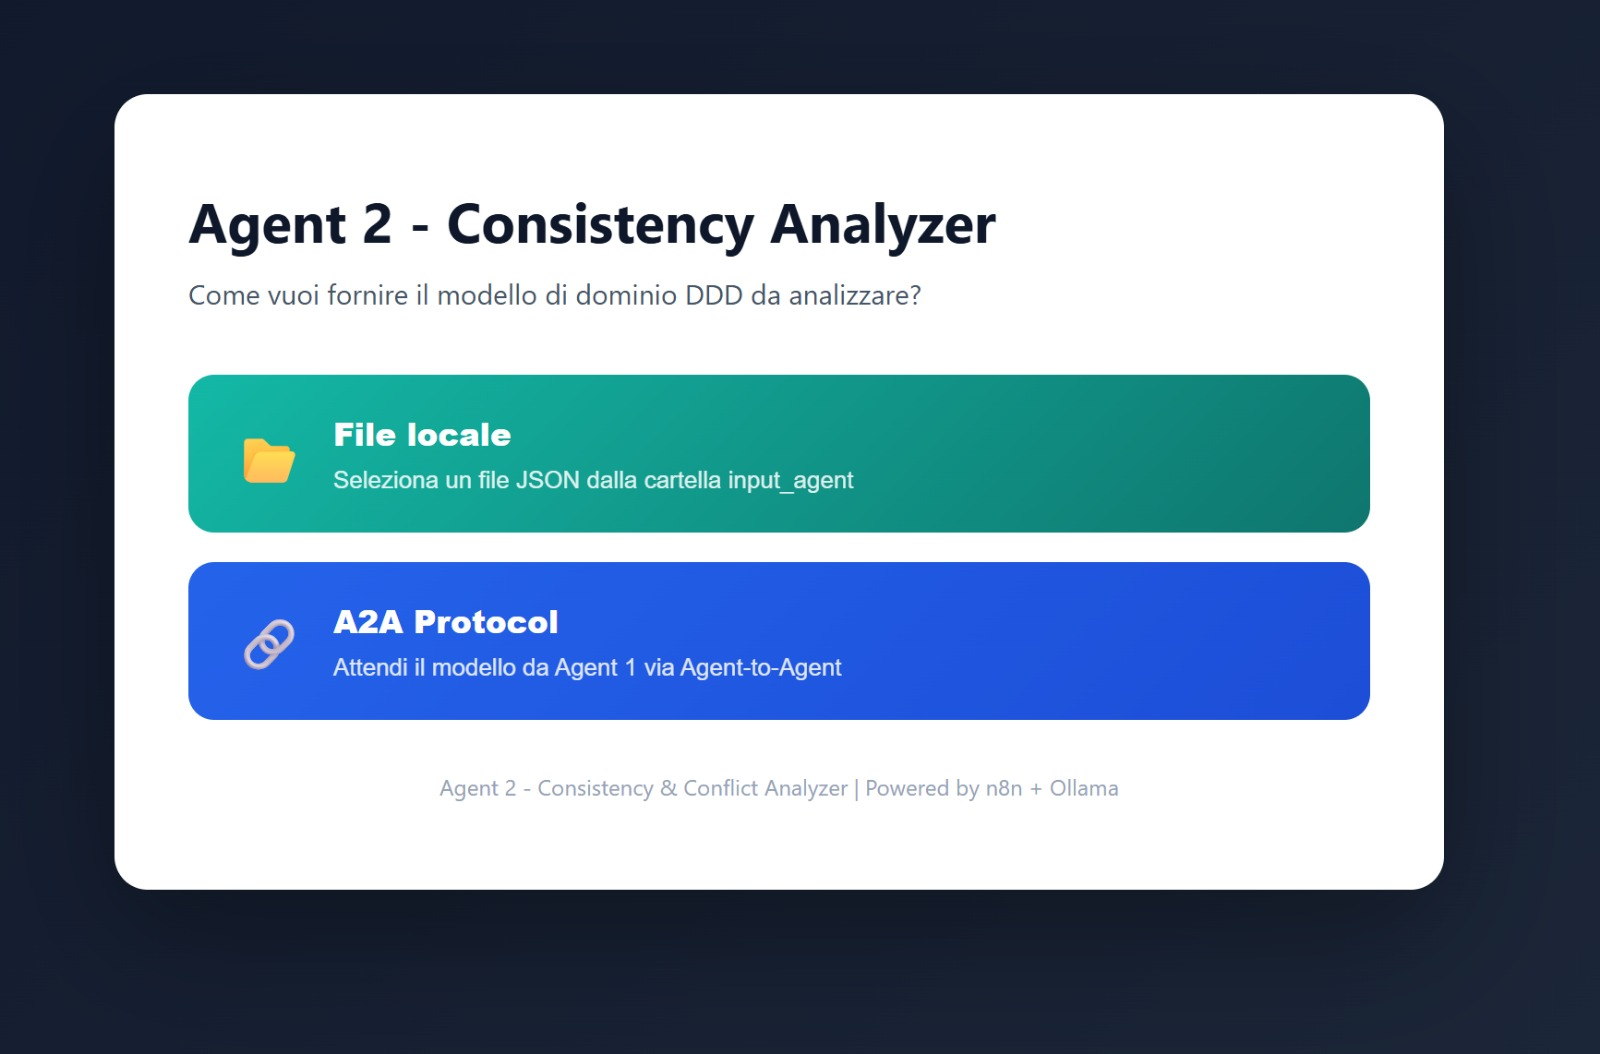
\includegraphics[width=0.80\textwidth]{open_page.png}
  \caption{Pagina iniziale dell'interfaccia web di Agent~2}
  \label{fig:open-page}
\end{figure}

% --- Step 2 ------------------------------------------------------------------
\subsection{Passo 2 --- Selezione del caso di test}

Scegliendo \textit{File locale}, l'interfaccia mostra automaticamente
tutti i file JSON disponibili nella cartella \texttt{input\_agent/},
con il relativo peso. L'utente clicca sul file che vuole analizzare.

\begin{figure}[H]
  \centering
  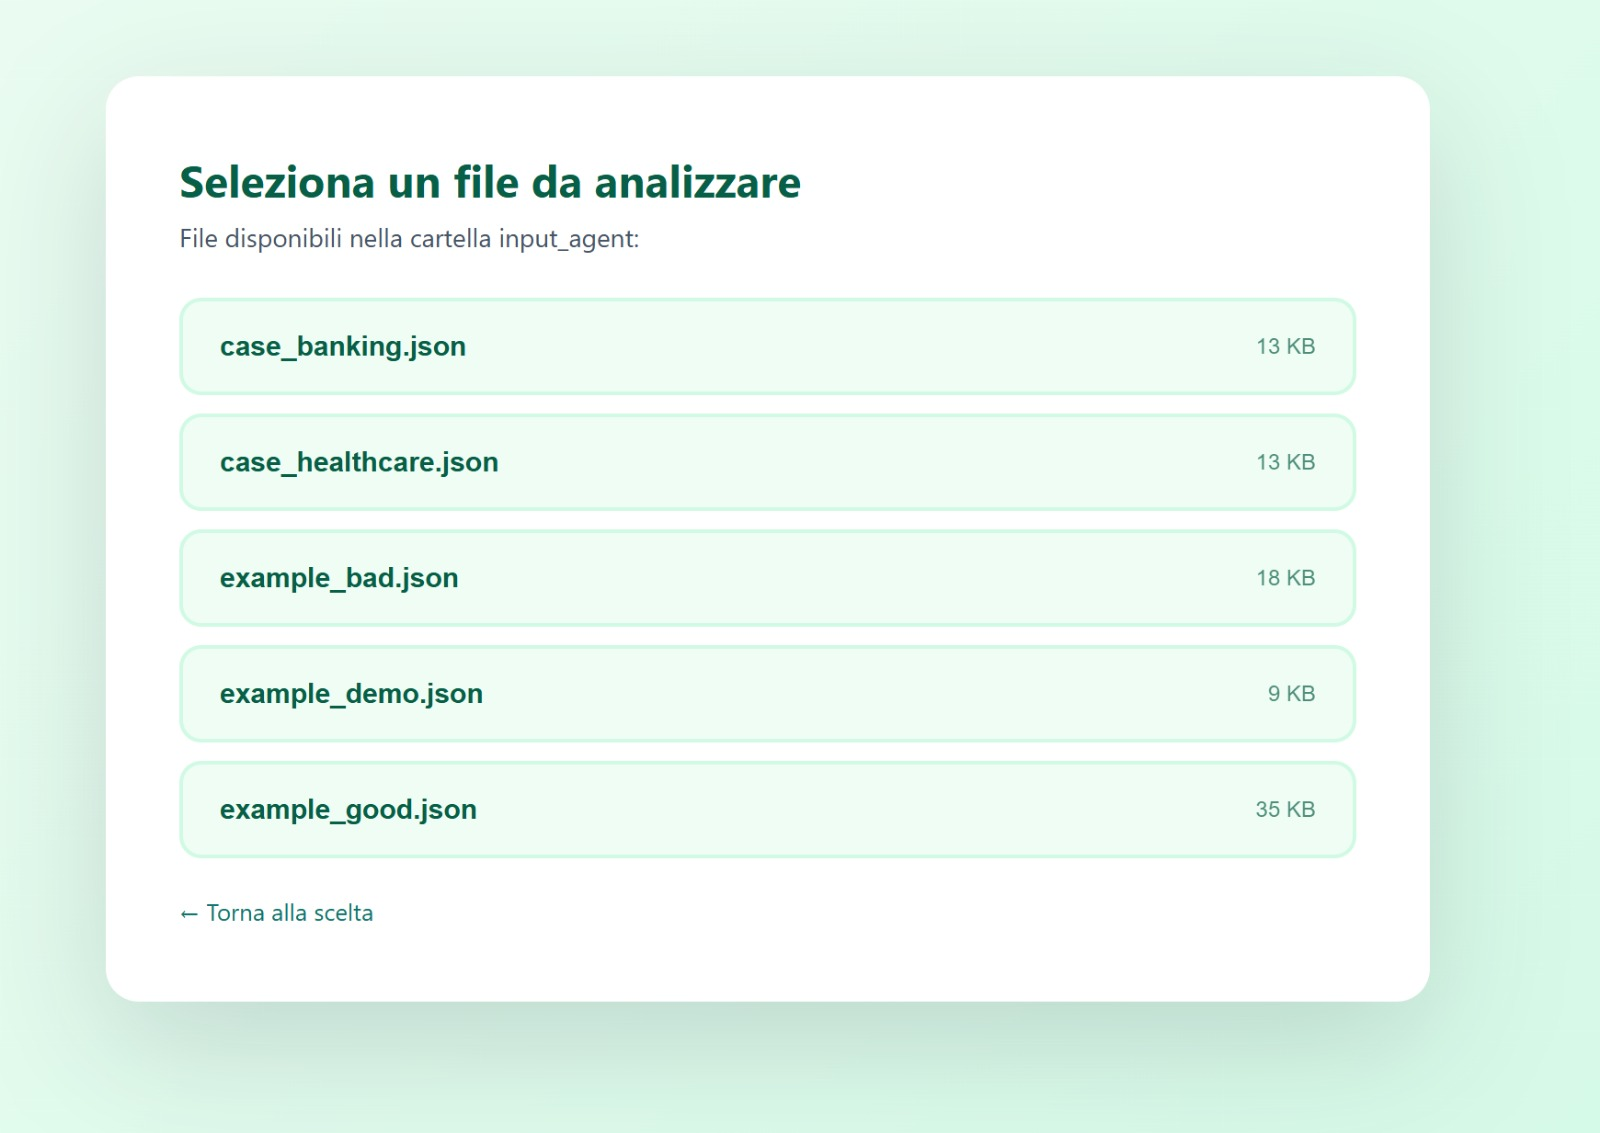
\includegraphics[width=0.80\textwidth]{scelta_json.png}
  \caption{Schermata di selezione del file JSON da analizzare}
  \label{fig:scelta-json}
\end{figure}

% --- Step 3 ------------------------------------------------------------------
\subsection{Passo 3 --- Analisi e domande di raffinamento}

Dopo la selezione, l'agente esegue l'analisi e presenta all'utente
una pagina di \textbf{validazione interattiva}. Per ogni problema rilevato
viene generata una domanda contestuale con risposte suggerite (radio button)
e la possibilità di inserire una risposta libera.

L'utente risponde a tutte le domande e clicca su \textit{Invia Risposte e Continua Raffinamento}:
il modello viene aggiornato e, se necessario, parte una nuova iterazione.
Il badge \textit{Iterazione N di M} in alto indica la progressione verso la convergenza.

\begin{figure}[H]
  \centering
  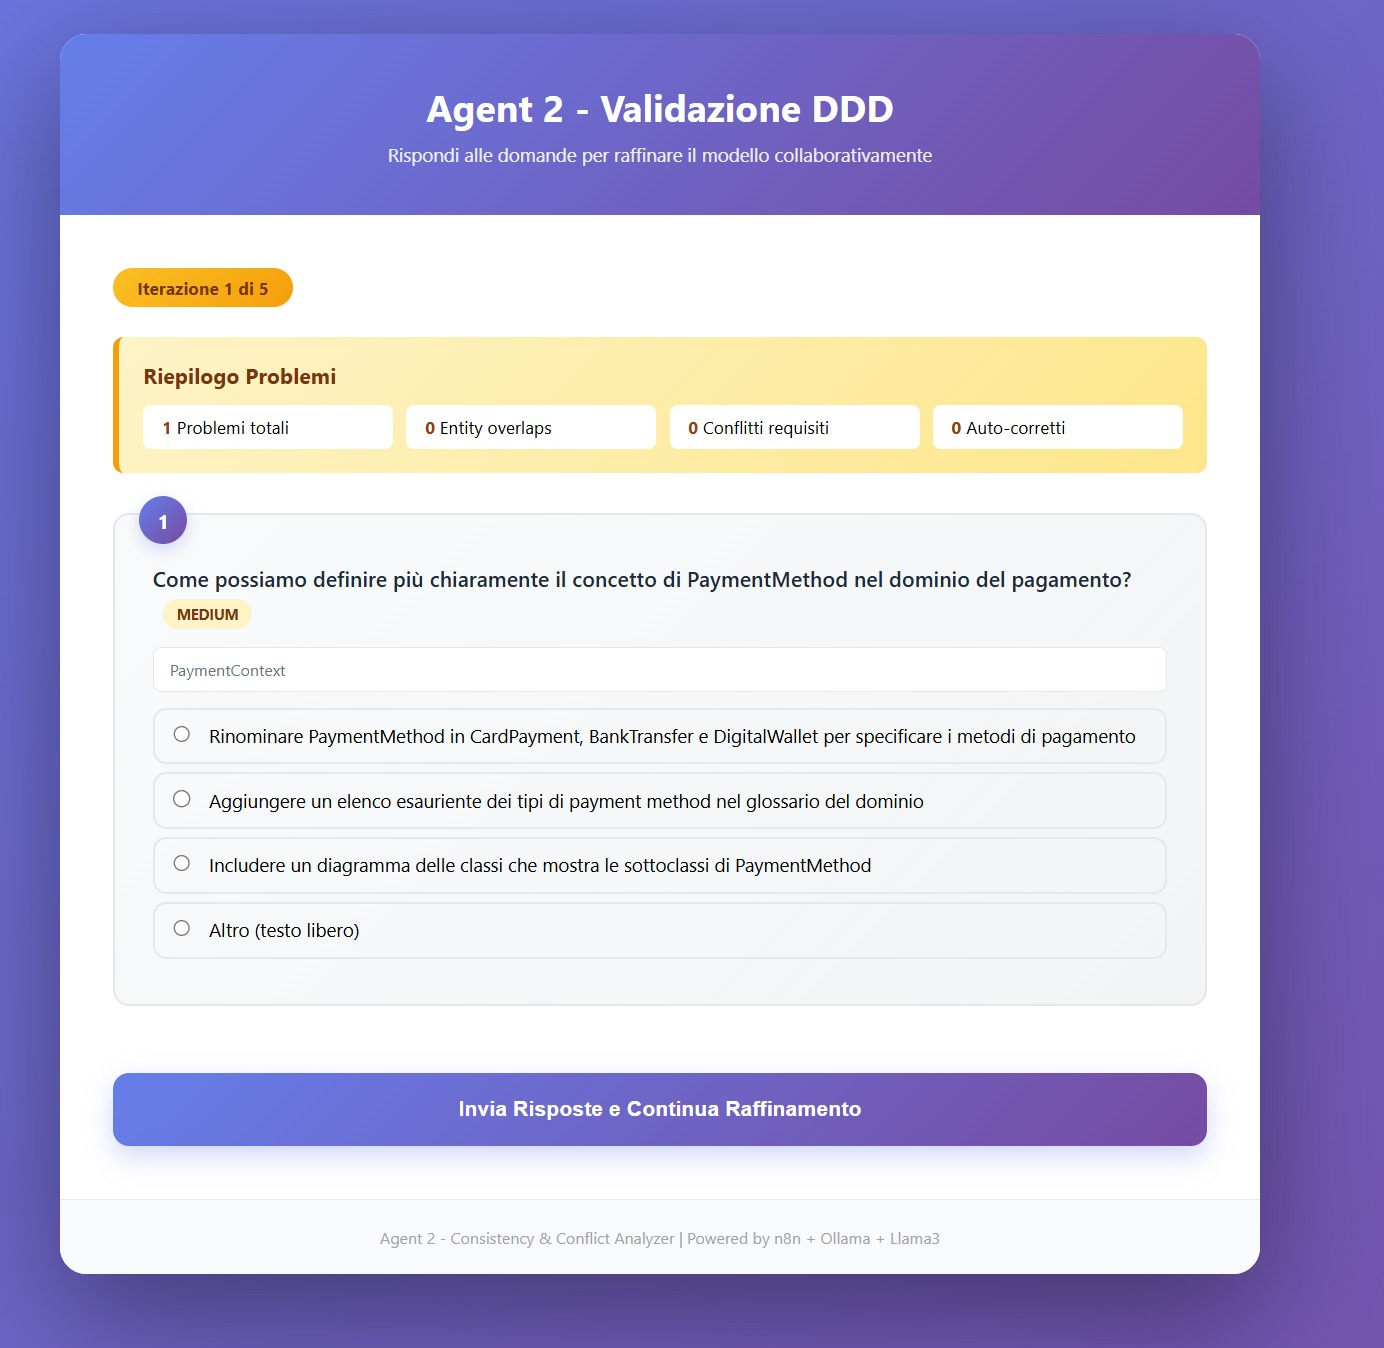
\includegraphics[width=0.80\textwidth]{domande.png}
  \caption{Schermata delle domande di raffinamento con riepilogo dei problemi rilevati}
  \label{fig:domande}
\end{figure}

Il ciclo si ripete finché tutti i problemi sono risolti e l'agente restituisce
lo stato \texttt{VALID}, oppure fino al raggiungimento del numero massimo di iterazioni
(calcolato adattativamente in base alla complessità del modello).

\end{document}

